% =============================================================================
% City Tour Planner — Prototype and Initial Design
% COMP.SE.110 Software Design, 2026–2027
%
% Build:   pdflatex City-Tour-Planner-Prototype-Design.tex   (run twice)
%      or: latexmk -pdf City-Tour-Planner-Prototype-Design.tex
% Engine:  pdfLaTeX. Only standard TeX Live packages are used.
% Fonts:   Helvetica clone (helvet, part of psnfss) — no custom fonts needed.
% Images:  figures/*.png (cropped screenshots). The uncropped Figma exports are
%          kept in figures/original/.
% =============================================================================
\documentclass[a4paper,10pt]{article}

% ---------- Encoding, font, typography ---------------------------------------
\usepackage[utf8]{inputenc}
\usepackage[T1]{fontenc}
\usepackage[scaled=0.92]{helvet}
\renewcommand{\familydefault}{\sfdefault}
\usepackage{courier}
\usepackage{microtype}

% ---------- Page layout --------------------------------------------------------
\usepackage[a4paper,top=2.3cm,bottom=2.0cm,left=1.9cm,right=1.9cm,
            headheight=15pt,headsep=0.6cm,footskip=1.0cm]{geometry}
\linespread{1.04}
\setlength{\parindent}{0pt}
\setlength{\parskip}{4.5pt plus 1pt minus 0.5pt}

\renewcommand{\topfraction}{0.9}
\renewcommand{\bottomfraction}{0.8}
\renewcommand{\textfraction}{0.08}
\renewcommand{\floatpagefraction}{0.75}
\setcounter{topnumber}{3}
\setcounter{totalnumber}{4}

% ---------- Colours ------------------------------------------------------------
\usepackage[table]{xcolor}
\definecolor{navy}{HTML}{14213D}
\definecolor{accent}{HTML}{14606B}
\definecolor{greytext}{HTML}{5B6670}
\definecolor{greyline}{HTML}{BCC3CA}
\definecolor{lightbg}{HTML}{EEF4F5}

% ---------- Graphics, tables, lists --------------------------------------------
\usepackage{graphicx}
\graphicspath{{figures/}{city-tour-planner-report-assets/figures/}}
\usepackage{booktabs}
\usepackage{array}
\usepackage{tabularx}
\usepackage[shortlabels]{enumitem}
\setlist{itemsep=1pt,topsep=2pt,parsep=0pt}
\newcolumntype{L}{>{\raggedright\arraybackslash}X}
\newcolumntype{Y}[1]{>{\raggedright\arraybackslash}p{#1}}
\renewcommand{\arraystretch}{1.22}
\setlength{\heavyrulewidth}{0.7pt}
\setlength{\lightrulewidth}{0.4pt}
\setlength{\tabcolsep}{5pt}

% ---------- Headings -----------------------------------------------------------
\usepackage{needspace}
\usepackage{titlesec}
\titleformat{\section}{\color{navy}\Large\bfseries}{\thesection}{0.6em}{}[{\color{greyline}\titlerule[0.5pt]}]
\titleformat{\subsection}{\color{accent}\normalsize\bfseries}{\thesubsection}{0.5em}{}
\titlespacing*{\section}{0pt}{11pt plus 3pt minus 2pt}{5pt plus 1pt}
\titlespacing*{\subsection}{0pt}{8pt plus 2pt minus 1pt}{2pt plus 1pt}

% ---------- Captions and custom float for the architecture diagram -------------
\usepackage{caption}
\usepackage{newfloat}
\usepackage{float}
\DeclareFloatingEnvironment[name=Diagram]{diagram}
\captionsetup{font={small,color=greytext},labelfont={bf,color=navy},
              labelsep=period,justification=raggedright,singlelinecheck=false}
\captionsetup[table]{skip=4pt}
\captionsetup[figure]{skip=5pt}
\captionsetup[diagram]{skip=5pt}

% ---------- Header and footer --------------------------------------------------
\usepackage{fancyhdr}
\usepackage{lastpage}
\pagestyle{fancy}
\fancyhf{}
\lhead{\small\color{greytext}City Tour Planner --- Prototype and Initial Design}
\rhead{\small\color{greytext}COMP.SE.110 Software Design, 2026--2027}
\cfoot{\small\color{greytext}Page \thepage\ of \pageref{LastPage}}
\renewcommand{\headrulewidth}{0.4pt}
\renewcommand{\headrule}{\hbox to\headwidth{\color{greyline}\leaders\hrule height \headrulewidth\hfill}}
\fancypagestyle{firstpage}{\fancyhf{}\cfoot{\small\color{greytext}Page \thepage\ of \pageref{LastPage}}\renewcommand{\headrulewidth}{0pt}}

% ---------- Diagram ------------------------------------------------------------
\usepackage{tikz}
\usetikzlibrary{arrows.meta,fit,backgrounds}

% ---------- Hyperlinks (load last) ---------------------------------------------
\usepackage[colorlinks=true,linkcolor=accent,urlcolor=accent,citecolor=accent,
            pdftitle={City Tour Planner --- Prototype and Initial Design},
            pdfauthor={Varun Ganesh Sondur, Pham Thanh, Georgios Malezoglou, Abdullah},
            pdfsubject={COMP.SE.110 Software Design, 2026--2027},
            bookmarksnumbered=true]{hyperref}

\begin{document}
\thispagestyle{firstpage}

% =============================================================================
% Title block
% =============================================================================
{\color{accent}\small\bfseries\MakeUppercase{COMP.SE.110 Software Design, 2026--2027}\par}
\vspace{2pt}
{\color{navy}\fontsize{26}{30}\selectfont\bfseries City Tour Planner\par}
\vspace{1pt}
{\color{navy}\Large Prototype and Initial Design\par}
\vspace{5pt}
{\color{accent}\rule{\linewidth}{1.1pt}\par}
\vspace{4pt}
{\small\color{greytext}\textbf{Submission:} Prototype and initial design\par}
{\small\color{greytext}\textbf{Team:} Varun Ganesh Sondur, Pham Thanh, Georgios Malezoglou, Abdullah\par}

% =============================================================================
\section{Project Overview}
% =============================================================================
City Tour Planner helps users plan a city visit around their available time and the weather. The user selects a city, date, start time, and tour duration. Our application combines information from external data sources and applies its own planning logic to suggest an ordered set of places to visit. The intended results are a map, an ordered list of stops, weather information, and relevant road traffic announcements when available.

We designed the application to support multiple cities rather than a single location. We used Helsinki as our initial location for investigating candidate APIs and understanding the available data. Our map and city-selection design allows us to extend the application to other cities using suitable data providers (Section~\ref{sec:multicity}).

\subsection{Main user workflow}
The user selects a city, date, start time, and tour duration. The application retrieves relevant weather, place, and traffic information, and we process the available data and apply our tour-planning rules. The planning logic selects and orders suitable places within the requested duration. The application then displays the itinerary, map, weather visualization, and available traffic information, and the user can show or hide data layers in the results view. Section~\ref{sec:flow} describes the technical request flow.

\subsection{Initial scope}
We intend the initial version to support tour planning for multiple cities using appropriate data providers, based on the selected date, start time, and duration. It filters and orders places with application-side logic, with weather-aware recommendations when suitable forecast data is available, and presents a map, an ordered list of suggested stops, weather visualization, and optional traffic information. It gives clear feedback when an external data source is unavailable.

Booking, payments, user accounts, live GPS tracking, and guaranteed optimal pedestrian routing are outside our initial scope. We will present walking times, train information, and precipitation probabilities as factual results only when a suitable data source supports them, and we will distinguish estimates from verified measurements.

% =============================================================================
\section{Data Sources and API Research}
% =============================================================================
\subsection{API Research Runner}
Before designing our integrations, we developed a separate \emph{API Research Runner} to test candidate endpoints. It records HTTP status codes, response times, content types, response previews, and errors in a JSON report. The endpoints we tested returned HTTP~200 during our initial research. This confirms that the requests succeeded at the HTTP level; it does not confirm that every field needed by our planning logic is available. The Runner is a development utility and not a production component of City Tour Planner.

\subsection{Tested data sources}
Table~\ref{tab:sources} summarizes the three sources we investigated and what each test does and does not establish.

\begin{table}[tbp]
\centering
\small
\caption{Data sources investigated with the API Research Runner.}
\label{tab:sources}
\rowcolors{2}{white}{lightbg}
\begin{tabularx}{\linewidth}{@{}Y{2.5cm}Y{2.35cm}L@{}}
\toprule
\rowcolor{white}\textbf{Source} & \textbf{Tested response} & \textbf{Planned use and limits} \\
\midrule
\textbf{FMI Open Data} (weather) & XML &
  Forecast measurements and timestamps for the weather chart and, where the data supports it, weather-aware place selection. We interpret each measurement by its actual unit and time coverage and do not assume that precipitation probability or any other field is available unless it is present in the retrieved data. \\
\textbf{Digitraffic} (road traffic) & JSON &
  Road traffic announcements as additional context for a tour. The tested endpoint provides road announcements only; it does not establish train departure times or delays. We treat rail information as outside the current integration unless we introduce and test a suitable additional source. \\
\textbf{Helsinki Service Map}\,\cite{servicemap,dataset} (places), \texttt{/unit/} endpoint & JSON &
  Place and service records. The data also contains general city services, so we filter records by category and relevant fields instead of treating every unit as a tourist attraction. Coverage is Helsinki and other municipalities in the Helsinki metropolitan area. \\
\bottomrule
\end{tabularx}
\end{table}

\subsection{Place data for multiple cities}\label{sec:multicity}
We designed the application around a \emph{selected city} and a provider integration layer instead of hard-coding Helsinki into the planning logic. The selected city determines which place-data provider we use, based on that provider's coverage. For cities outside the Service Map's coverage, our design allows us to integrate alternative providers that supply relevant place data, without redesigning the workflow. Our API tests so far used Helsinki as the starting location; additional city providers are part of our planned implementation.

\subsection{Combining the data}
The external APIs supply raw information, and our application turns it into a proposed itinerary. We (1)~identify the data sources available for the selected city, (2)~retrieve the relevant weather, place, and traffic information, (3)~normalize provider-specific responses into application-level models, (4)~filter places according to our planning rules, and (5)~select and order stops within the requested duration. We keep provider-specific processing separate from the planning logic, distinguish real provider data from estimates, and handle missing information explicitly instead of inventing values.

% =============================================================================
\section{Technologies and Architecture}
% =============================================================================
\subsection{Planned technologies}
Table~\ref{tab:tech} lists our main technology direction. We will select the final HTTP integration and charting libraries according to the needs of the implementation.

\begin{table}[tbp]
\centering
\small
\caption{Planned technology stack.}
\label{tab:tech}
\rowcolors{2}{white}{lightbg}
\begin{tabularx}{\linewidth}{@{}Y{3.1cm}Y{5.6cm}L@{}}
\toprule
\rowcolor{white}\textbf{Area} & \textbf{Technology} & \textbf{Intended use} \\
\midrule
Backend & Java 22, Spring Boot 3.5.6 & Application workflow and tour-planning logic \\
Build, configuration & Maven; YAML, Jackson & Dependency management and builds; configuration and JSON processing \\
API communication & Java HTTP Client or Spring HTTP support & External API requests \\
Data providers & FMI Open Data, Digitraffic, Helsinki Service Map and additional providers & Weather, road traffic, and place data for supported cities \\
Frontend & React with Vite & Planning form and results interface \\
Map & Leaflet with OpenStreetMap tiles (proposed) & Places and suggested stop sequence \\
Charts & Recharts or Chart.js & Weather visualization \\
Frontend--backend & REST API, JSON, browser \texttt{fetch} & Communication with the Java backend \\
UI prototype & Figma & Screen designs and prototype interactions \\
\bottomrule
\end{tabularx}
\end{table}

\subsection{Main components}
We separate the frontend, application workflow, tour-planning logic, and external API integrations (Table~\ref{tab:components}).

\begin{table}[tbp]
\centering
\small
\caption{Main software components and their responsibilities.}
\label{tab:components}
\rowcolors{2}{white}{lightbg}
\begin{tabularx}{\linewidth}{@{}Y{3.1cm}L@{}}
\toprule
\rowcolor{white}\textbf{Component} & \textbf{Responsibility} \\
\midrule
React frontend & Collects the city, date, start time, and duration; displays the loading state, itinerary, map, weather chart, and traffic information when available; provides controls for showing and hiding data layers. \\
Application layer & Receives and validates tour requests, coordinates data retrieval and planning, and returns the generated result to the frontend. \\
Tour-planning logic & Filters places using the available data and user selections, applies weather-aware rules where supported, and selects and orders stops within the requested duration. \\
Provider interfaces and adapters & Isolate external API requests and convert provider-specific responses into application-level models. \\
External providers & Initially FMI (weather), Helsinki Service Map and additional providers (places), and Digitraffic (road traffic announcements). \\
\bottomrule
\end{tabularx}
\end{table}

\subsection{Component interaction and request flow}\label{sec:flow}
Diagram~\ref{dia:arch} shows the component structure we propose. It describes the architecture we intend to implement, not a claim that every component is already complete. The numbered steps below describe the request flow.

\begin{diagram}[tbp]
\centering
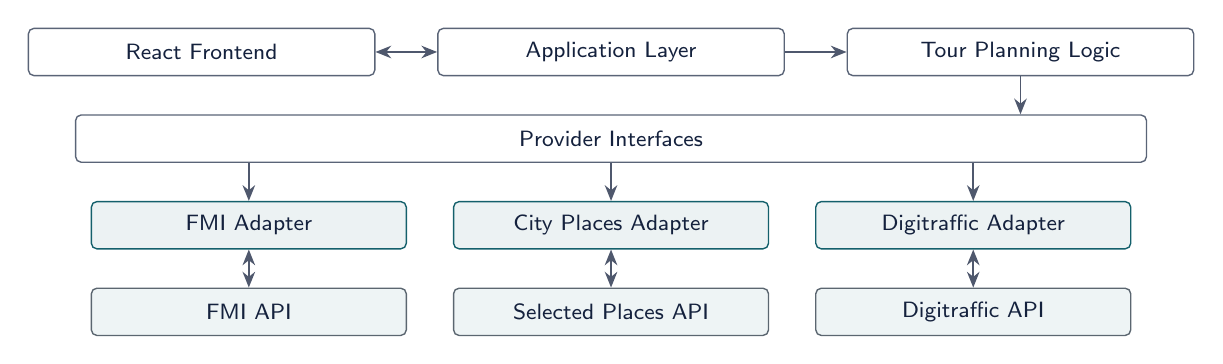
\begin{tikzpicture}[
  box/.style={draw=navy!70, fill=white, rounded corners=2pt, minimum height=6mm,
              align=center, font=\footnotesize, text=navy, line width=0.5pt, inner sep=3pt},
  top/.style={box, minimum width=4.4cm},
  adp/.style={box, draw=accent, fill=accent!8, minimum width=4.0cm},
  ext/.style={box, draw=greytext, fill=lightbg, minimum width=4.0cm},
  arr/.style={-{Stealth[length=2mm,width=1.6mm]}, line width=0.6pt, draw=navy!75},
  biarr/.style={{Stealth[length=2mm,width=1.6mm]}-{Stealth[length=2mm,width=1.6mm]}, line width=0.6pt, draw=navy!75}
]
  \node[top] (ui)   at (-5.2,0) {React Frontend};
  \node[top] (app)  at (0,0)    {Application Layer};
  \node[top] (plan) at (5.2,0)  {Tour Planning Logic};
  \node[box, minimum width=13.6cm] (prov) at (0,-1.1) {Provider Interfaces};
  \node[adp] (w) at (-4.6,-2.2) {FMI Adapter};
  \node[adp] (p) at (0,-2.2)    {City Places Adapter};
  \node[adp] (t) at (4.6,-2.2)  {Digitraffic Adapter};
  \node[ext] (wa) at (-4.6,-3.3) {FMI API};
  \node[ext] (pa) at (0,-3.3)    {Selected Places API};
  \node[ext] (ta) at (4.6,-3.3)  {Digitraffic API};

  \draw[biarr] (ui) -- (app);
  \draw[arr] (app) -- (plan);
  \draw[arr] (plan.south) -- (plan.south |- prov.north);
  \draw[arr] (w.north |- prov.south) -- (w.north);
  \draw[arr] (p.north |- prov.south) -- (p.north);
  \draw[arr] (t.north |- prov.south) -- (t.north);
  \draw[biarr] (w) -- (wa);
  \draw[biarr] (p) -- (pa);
  \draw[biarr] (t) -- (ta);
\end{tikzpicture}
\caption{Component interaction. Single-headed arrows show the direction of control; double-headed arrows show request and response exchanges.}
\label{dia:arch}
\end{diagram}

\begin{enumerate}[noitemsep,leftmargin=1.6em,midpenalty=10000]
  \item The user submits a tour request through our frontend.
  \item The backend validates the request and identifies the data providers suitable for the selected city.
  \item Our integration layer retrieves the relevant weather, place, and traffic data.
  \item Provider adapters normalize the responses into application-level models.
  \item Our planning logic filters and orders candidate places.
  \item The backend returns the itinerary and visualization data.
  \item The frontend displays the results and any relevant data-availability messages.
\end{enumerate}

We separate these layers so that the planning logic does not depend on the response formats of individual providers and so that we can add or replace a data source as city support grows. The workflow also tolerates partial data availability: if one provider fails, the application can explain the limitation and use other suitable data where possible, instead of silently treating missing information as valid.

% =============================================================================
\Needspace{6\baselineskip}
\section{Design Approach}
% =============================================================================
\subsection{Adapter pattern}
We chose the Adapter pattern as our main approach for integrating external providers that have different endpoints and response formats. For example, we can use \texttt{FmiWeatherAdapter}, \texttt{ServiceMapPlacesAdapter}, other city-specific place adapters, and \texttt{DigitrafficAdapter}. Each adapter converts the corresponding external response into our application's data models. This keeps provider-specific details out of the tour-planning logic and supports our multi-city design, because we can add or replace a place provider without rewriting the planning workflow. Related constraints carry into the implementation: we select providers per city instead of assuming one source covers every location, we filter general service records into relevant places, we use forecast values according to their actual units, timestamps, and coverage, and we treat road traffic announcements separately from train schedules and delays.

\subsection{Strategy pattern}
We may need different selection rules for general, indoor-focused, and outdoor-focused tours. If these rules become sufficiently different, we can represent them through a common strategy interface. For the initial version, we intend to keep the planning logic proportionate to the requirements and to introduce separate strategy implementations only where they improve the design.

% =============================================================================
\Needspace{6\baselineskip}
\section{UI Prototype}
% =============================================================================
Our Figma prototype\,\cite{figma} demonstrates the intended user journey from entering tour preferences to reviewing the suggested itinerary. The figures below are screenshots exported from the prototype; we cropped only empty space at the bottom of each screen. The weather values (70\% chance of rain, 6\,\textdegree C, 4\,m/s wind), stop times, walking times, route lines, and traffic announcements in these screens are illustrative prototype content. The prototype marks the map as a placeholder for Leaflet and the traffic rows as sample text. We do not present any of these values as live or verified data.

\subsection{Planning screen}
The planning screen (Figure~\ref{fig:planning}) provides a city selector, date, start time, tour-duration options (2\,h, 4\,h, 6\,h), and a \emph{Generate Tour} action. The panel on the left introduces the main features: weather information, traffic information, places, and the proposed tour. The selected city determines which data providers the backend uses, which reflects our decision to design the application for multiple cities. The introductory text on this screen mentions train information; as described in Section~\ref{sec:multicity} and Table~\ref{tab:sources}, the Digitraffic endpoint we tested covers road announcements only, and rail information is outside our current integration.

\begin{figure}[tbp]
\centering
\includegraphics[width=0.72\linewidth]{planning-screen.png}
\caption{City Tour Planner planning screen.}
\label{fig:planning}
\end{figure}

\subsection{Loading screen}
The loading screen (Figure~\ref{fig:loading}) communicates progress while data is retrieved. It lists weather, road traffic, and places as separate retrieval steps with their own status (\emph{Done}, \emph{Loading}, \emph{Waiting}), so users can see what the application is processing. In the implementation, these indicators will reflect actual request states, and we intend to handle failed or delayed requests without leaving the user waiting indefinitely.

\begin{figure}[tbp]
\centering
\includegraphics[width=0.72\linewidth]{loading-screen.png}
\caption{Loading state showing progress across data sources.}
\label{fig:loading}
\end{figure}

\subsection{Results screen}
The results screen (Figure~\ref{fig:results}) brings the outputs together: a map with numbered stops and a suggested visit sequence, a stop list with names, categories, and planned times, an hourly weather chart with a tour-window indicator, and a \emph{Why this tour} panel that explains how the weather influenced the suggested tour. Road traffic announcements appear in a separate table when available. The \emph{Data layers} panel lets the user switch the weather, transport, and places layers on and off; the prototype specifies that switching a layer updates the view instantly, without new API calls.

\begin{figure}[tbp]
\centering
\includegraphics[width=0.70\linewidth]{results-screen.png}
\caption{Results screen with the map, weather information, and place layers.}
\label{fig:results}
\end{figure}

\subsection{Unavailable-traffic state}
We also designed a results state in which traffic announcements are unavailable (Figure~\ref{fig:notraffic}). A notice states that the Digitraffic road announcements are unavailable and that the tour is shown without traffic information, and the transport layer is switched off. This demonstrates how the application communicates a missing data source instead of silently presenting unavailable information as valid, a behavior that the standard results screen does not show.

\begin{figure}[tbp]
\centering
\includegraphics[width=0.70\linewidth]{unavailable-traffic.png}
\caption{Results screen demonstrating unavailable traffic information.}
\label{fig:notraffic}
\end{figure}

% =============================================================================
\section{Team Contributions and AI Usage}
% =============================================================================
\subsection{Team contributions}
We have provisionally divided the work by area so that we can develop the application in parallel while coordinating integration (Table~\ref{tab:team}). We will adjust responsibilities when needed, and all members review the overall design.

\begin{table}[H]
\centering
\small
\caption{Provisional allocation of responsibilities.}
\label{tab:team}
\rowcolors{2}{white}{lightbg}
\begin{tabularx}{\linewidth}{@{}Y{3.0cm}Y{3.3cm}L@{}}
\toprule
\rowcolor{white}\textbf{Member} & \textbf{Main area} & \textbf{Contribution and planned responsibilities} \\
\midrule
\textbf{Varun Ganesh Sondur} & Backend architecture and API integration &
  Built the API Research Runner, investigated external API feasibility, and contributed to project planning and architecture. Will focus on provider adapters, backend integration, and tour-planning logic. \\
\textbf{Pham Thanh} & Frontend and UI &
  Designed the Figma prototype and contributed the screen content based on API findings. Will focus on the planning form, results layout, map, weather chart, data-layer controls, and frontend--backend integration. \\
\textbf{Georgios Malezoglou} & Tour-planning logic and data processing &
  Will help define place filtering, weather-aware selection rules, stop ordering, duration estimates, and tests for planning behavior. \\
\textbf{Abdullah} & Testing and integration support &
  Will help test API and application behavior, check city-specific data integration, test unavailable-data scenarios, and coordinate technical documentation and integration checks. \\
\bottomrule
\end{tabularx}
\end{table}

\subsection{AI tool usage disclosure}
We used AI tools as part of our project preparation and development workflow, including exploring design options, supporting spec-driven development, reviewing and optimizing code, and considering architectural and implementation decisions. Our use of these tools supported the development process rather than replacing our own technical judgment.

We treat AI-generated suggestions as input rather than automatically accepting them. We review relevant outputs, consider design trade-offs, and check technical claims against API responses, available documentation, and implementation tests where applicable. We remain responsible for our final requirements, design decisions, code, and submitted work. This disclosure describes our collective workflow; any tool-specific attribution or additional AI use is documented according to the work actually performed by the team.

% =============================================================================
\section{Conclusion}
% =============================================================================
We designed City Tour Planner as a multi-city tour-planning application that combines weather, place, and traffic information with our own planning logic. We tested candidate APIs with Helsinki as our starting location and designed the application so that additional cities can be supported through suitable data providers.

Our proposed architecture separates the frontend, application workflow, planning logic, and provider integrations, with the Adapter pattern isolating external API formats, which keeps API details out of itinerary generation and makes the application easier to extend. Our Figma prototype demonstrates the planning workflow, loading feedback, results visualization, and handling of unavailable traffic information.

Our next implementation steps are to connect the agreed components, build the planning logic, integrate the frontend with the backend, and test the application against real API responses. We will use these tests to refine the itinerary and to ensure that the displayed information accurately reflects the available data.

% =============================================================================
% =============================================================================
\renewcommand{\refname}{References}
\begin{thebibliography}{9}
\setlength{\itemsep}{2pt}
\small
\bibitem{servicemap} Helsinki Service Map API documentation. \href{https://www.hel.fi/palvelukarttaws/restpages/ver4.html}{\nolinkurl{https://www.hel.fi/palvelukarttaws/restpages/ver4.html}}
\bibitem{dataset} Service Map dataset information. \href{https://avoindata.suomi.fi/data/en_GB/dataset/paakaupunkiseudun-palvelukartan-rest-rajapinta}{\nolinkurl{https://avoindata.suomi.fi/data/en_GB/dataset/paakaupunkiseudun-palvelukartan-rest-rajapinta}}
\bibitem{figma} City Tour Planner Prototype, Figma. \href{https://www.figma.com/proto/xLJSzzdVMFzEHprbCb2SrW/City-Tour-Planner-Prototype?node-id=0-1&t=c8UDhzHjZfPHAGFD-1}{Open the Figma prototype}
\end{thebibliography}

\end{document}
